\section{Experiments}
\label{sec:experiments}

The operation of the \emph{graph} module was tested using
Mininet, a simulation system created exactly to simulate SDN
scenarios~\cite{lantz2010network}. We had to extend Mininet with
methods to control the addition and removal of network elements,
so we could observe the system behavior as the topology changes
dynamically.

Besides the code interfaces, which affected different classes,
the standard command interface \emph{prompt} was extended with new commands
to dynamically add/remove controllers, switches, hosts, links and network
interfaces. All changes were made with compatibility in mind, so the
original Mininet data structures and interfaces were preserved as much as
possible.

The goal of the experiments that follow was to validate and evaluate the
performance of the proposed system.
Consider a network with a simple topology as shown in
Figure~\ref{fig:topology}, that has two switches,
each with three hosts;
there is an edge (link) between the switches, and
one instance of the POX controller controls both switches.

\begin{figure}[!h]
    \centering
    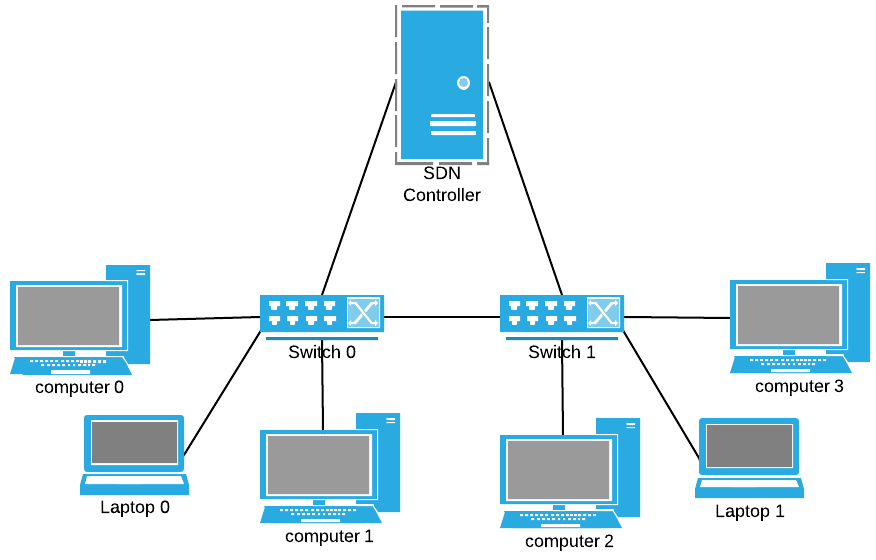
\includegraphics[width=1.0\columnwidth]{img/simple_topology.png}
    \caption{Simple topology}
    \label{fig:topology}
\end{figure}


\subsection{Entity Detection}

When the system starts, the graph is empty. 
The switches are the first entities to be identified, because
the controller is directly connected to the switches 
through the OpenFlow interface and it sees nothing before those connections
are established. A \emph{ConnectionUp} event is
triggered at the controller core. Figure~\ref{fig:detection} shows the
events logged during the start of the execution.

\begin{figure}[h!]
\centering
\begin{lstlisting}
INFO:topology.graph:SwitchJoin id: 2
INFO:topology.graph:SwitchJoin id: 1
INFO:topology.graph:1, 2
DEBUG:openflow.discovery:Dropping LLDP packet 275
INFO:topology.graph:LinkEvent fired
INFO:host_tracker:Learned 1 1 7e:e6:9b:89:39:2e got IP 10.0.0.1
INFO:topology.graph:HostJoin id: 7e:e6:9b:89:39:2e
INFO:host_tracker:Learned 2 1 62:77:44:24:13:49 got IP 10.0.0.2
INFO:topology.graph:HostJoin id: 62:77:44:24:13:49
\end{lstlisting}
\caption{Entity Detection}
\label{fig:detection}
\end{figure}

In the first two lines of the log shown in Figure~\ref{fig:detection},
the graph module was notified 
about the discovery of two switches in the network.
Therefore, two vertexes of the switch entity type were 
referenced in the graph.
Line 4 indicates one event related to LLDP, when switches start to look for
others, and \emph{of.discovery} is activated. Right after that,
in line 5, we notice the discovery of a link (between switches).
Lines 7 and 9 show two hosts discovered by \emph{topology}, as a result
of them being discovered by the \emph{host\_tracker} module, possibly
during their fist effort to connect to the DHCP server.
Any new package that passes through a switch and has no installed flow in the
flow table is forwarded to the controller, that triggers a \emph{PacketIn}
event and identifies the entities (hosts and switches) involved in the
communication.
By continuing acting like this, the network entities are identified and
represented in the graph.

\subsection{Removing Entities}

Two experiments were executed to observe how the graph was updated when an
entity became unavailable. For the event of host removal, we turned off one
host's network interface using the Mininet command prompt. The
\emph{host\_tracker} module, in the absence of traffic from a certain host,
triggers a timer event and an ARPRequest message is sent to the missing
host. The module uses a two-out-of-three policy to decide if a host is
down. By doing so, after thirty seconds the host was marked as unavailable
and a \emph{HostLeave} event was triggered, updating the graph.

For the second experiment, a switch was turned off using Mininet. Since the
controller had a direct connection to the switch (for the OpenFlow
protocol), once the POX \emph{core} detected the loss of the connection to
the switch, the graph was updated, removing the switch and hosts connected
to it.


\subsection{Real-time visualization}

Figure~\ref{fig:full_graph} shows the graph of a network  with 8 switches,
each one with 30 hosts connected, totalizing 248 network entities.
This graph was updated in real time by events that occurred inside the
controller, like entities joining/leaving, observation of traffic volume
in the network, and others.

\begin{figure}[htb!]
    \centering
    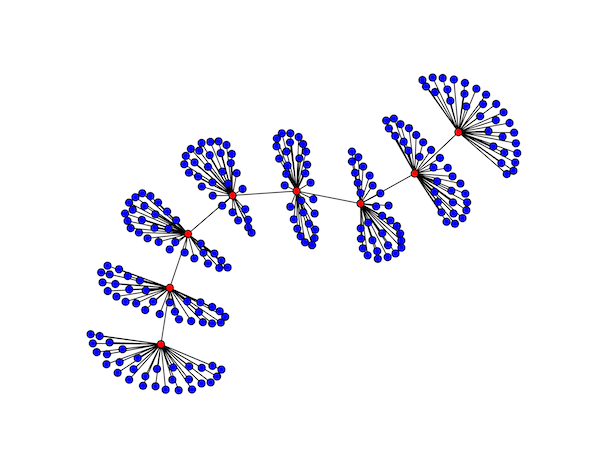
\includegraphics[width=1.0\columnwidth]{img/full_graph.png}
    \caption{248 nodes network represented by a graph}
    \label{fig:full_graph}
\end{figure}

Events were programmed to occur during a predefined interval and the final
graph was obtained within seconds of the end of the series of add/remove
commands. As observed previously with the individual events, host removals
were detected withing 30 seconds, host additions were detected in
milliseconds after their first transmission, and switch events were
detected promptly as the OpenFlow connections went up/down.


\subsection{Network Traffic Identification}

We used the Iperf tool as a server on host 'Host 0a' 
to compute the (TCP) traffic on the network shown in Figure~\ref{fig:iperf}.
The host 'Host 1e' connected as a client.
As can be seen in Figure~\ref{fig:iperf}, the traffic 
in bytes on the edges that connect those hosts is larger than that of 
the other hosts.
In the moment that the port counters were read and the 
edges weights computed, the traffic was 55894 bytes through the path 
between the two hosts.

The values observed for the other links (41 bytes) are from the ARP
messages sent by those hosts and 
by \emph{host\_tracker}.
The experiment with Iperf shows a forwarding rate (throughput) 
between hosts of 300 Megabits per second, confirming there is no bottleneck
due to the graph abstraction.

\begin{figure}[htb!]
    \centering
    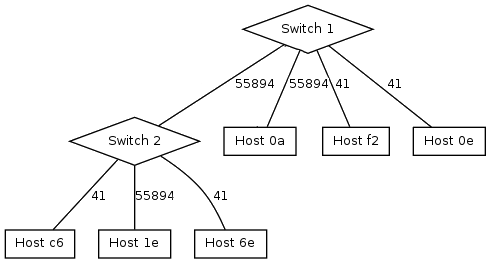
\includegraphics[width=1.0\columnwidth]{img/graph_iperf.png}
    \caption{TCP Traffic (number of bytes) between the hosts 'Host 1e' and 'Host 0a'}.
    \label{fig:iperf}
\end{figure}

\subsection{Minimum Spanning Tree}

Minimum spanning trees are essential in many tasks in network management.
Tasks like trigger 'alarms' when the tree is disconnected or 
loops are detected, as presented are essential~\cite{schmid2013exploiting}.
One can think of a distributed system that uses such a tree to 
execute a message propagation algorithm using flooding to limit the
number of retransmissions~\cite{Monsanto:2013:CSN:2482626.2482629}.
A network with multiple paths can implement dynamic load balancing by
computing multiple spanning trees in real time~\cite{spain}.

The minimum spanning tree algorithm implemented in the \emph{graph} module
was tested by using it to maintain
a dynamic minimum spanning tree as the network was updated.
Whenever the graph was altered by the addition/removal of an edge/vertex in
response to a change in the underlying topology, the minimum spanning tree
was re-computed as expected.
